\documentclass[charterfonts,lotsofwhite]{patmorin}
\usepackage{graphicx}

\newcommand{\chain}[2]{[#1#2]}
\newcommand{\dual}[1]{\varphi(#1)}
\newcommand{\parity}{\textsc{Colored-Parity}}

%\newcommand{\email}[1]{\texttt{#1}}
% Avoid line breaks before citations (\cite) and references (\ref)
%\let\latexcite=\cite
%\def\cite{\nolinebreak\latexcite}
%\let\latexref=\ref
%\def\ref{\nolinebreak\latexref}

 
%\usepackage{amsthm}

\newcommand{\centeripe}[1]{\begin{center}\Ipe{#1}\end{center}}
\newcommand{\comment}[1]{}

\newcommand{\centerpsfig}[1]{\centerline{\psfig{#1}}}

\newcommand{\seclabel}[1]{\label{sec:#1}}
\newcommand{\Secref}[1]{Section~\ref{sec:#1}}
\newcommand{\secref}[1]{\mbox{Section~\ref{sec:#1}}}

\newcommand{\alglabel}[1]{\label{alg:#1}}
\newcommand{\Algref}[1]{Algorithm~\ref{alg:#1}}
\newcommand{\algref}[1]{\mbox{Algorithm~\ref{alg:#1}}}

\newcommand{\applabel}[1]{\label{app:#1}}
\newcommand{\Appref}[1]{Appendix~\ref{app:#1}}
\newcommand{\appref}[1]{\mbox{Appendix~\ref{app:#1}}}

\newcommand{\tablabel}[1]{\label{tab:#1}}
\newcommand{\Tabref}[1]{Table~\ref{tab:#1}}
\newcommand{\tabref}[1]{Table~\ref{tab:#1}}

\newcommand{\figlabel}[1]{\label{fig:#1}}
\newcommand{\Figref}[1]{Figure~\ref{fig:#1}}
\newcommand{\figref}[1]{\mbox{Figure~\ref{fig:#1}}}

\newcommand{\eqlabel}[1]{\label{eq:#1}}
\newcommand{\eqref}[1]{(\ref{eq:#1})}

\newtheorem{thm}{Theorem}{\bfseries}{\itshape}
\newcommand{\thmlabel}[1]{\label{thm:#1}}
\newcommand{\thmref}[1]{Theorem~\ref{thm:#1}}

\newtheorem{lem}{Lemma}{\bfseries}{\itshape}
\newcommand{\lemlabel}[1]{\label{lem:#1}}
\newcommand{\lemref}[1]{Lemma~\ref{lem:#1}}

\newtheorem{cor}{Corollary}{\bfseries}{\itshape}
\newcommand{\corlabel}[1]{\label{cor:#1}}
\newcommand{\corref}[1]{Corollary~\ref{cor:#1}}

\newtheorem{obs}{Observation}{\bfseries}{\itshape}
\newcommand{\obslabel}[1]{\label{obs:#1}}
\newcommand{\obsref}[1]{Observation~\ref{obs:#1}}

\newtheorem{assumption}{Assumption}{\bfseries}{\rm}
\newenvironment{ass}{\begin{assumption}\rm}{\end{assumption}}
\newcommand{\asslabel}[1]{\label{ass:#1}}
\newcommand{\assref}[1]{Assumption~\ref{ass:#1}}

\newcommand{\proclabel}[1]{\label{alg:#1}}
\newcommand{\procref}[1]{Procedure~\ref{alg:#1}}

\newtheorem{rem}{Remark}
\newtheorem{op}{Open Problem}

\newcommand{\etal}{\emph{et al}}

\newcommand{\voronoi}{Vorono\u\i}
\newcommand{\ceil}[1]{\left\lceil #1 \right\rceil}
\newcommand{\floor}[1]{\left\lfloor #1 \right\rfloor}



% Start of patch
%\def\more-auths{%
%\end{tabular}
%\begin{tabular}{c}}
% End of patch

\newcommand{\email}[1]{\texttt{#1}}

%%%%%%%%%%%%%%%%%%%%%%%%%%%%%%%%%%%%%%%%%%%%%%%%%%%%%%%%%%%%%%%%%%%%%%%%%%%%%%

\begin{document}
\title{\MakeUppercase{Geodesic Ham-Sandwich Cuts}%
  \thanks{Partially supported by  NSERC, NSF, DURSI 2001SGR00224, Acció Integrada
UPC-McGill (DURSI2004) and MCYT BFM2003-0368.}}
\author{Prosenjit Bose%
	\thanks{School of Computer Science, Carleton University,
		\email{jit@cs.carleton.ca}}
   \and Erik D. Demaine%
	\thanks{MIT Laboratory for Computer Science, 
		\email{edemaine@mit.edu}}
   \and Ferran Hurtado%
	\thanks{Departament de Matem\`atica Aplicada II, 
		Universitat Polit\`ecnica de Catalunya, 
		\email{Ferran.Hurtado@upc.es}}
   \and John Iacono%
        \thanks{Department of Computer and Information Sciences,
		Brooklyn Polytechnic University,
		\email{jiacono@poly.edu}}
   \and Stefan Langerman%
	\thanks{Charg\'e de recherches du FNRS, 
		D\'epartement d'Informatique,
		Universit\'e Libre de Bruxelles,
		\email{stefan.langerman@ulb.ac.be}}
   \and Pat Morin%
        \thanks{School of Computer Science, Carleton University,
		\email{morin@cs.carleton.ca}}
}
\date{}
\maketitle

\begin{abstract} Let $P$ be a simple polygon with $m$ vertices, $k$ of
which are reflex, and which contains $r$ red points and $b$ blue
points in its interior.  Let $n=m+r+b$. A \emph{ham-sandwich geodesic}
is a shortest path in $P$ between any two points on the boundary of
$P$ that simultaneously bisects the red points and the blue points.
We present an $O(n \log k)$-time algorithm for finding a ham-sandwich
geodesic.  We also show that this algorithm is optimal in the
algebraic computation tree model when parameterizing the running time
with respect to $n$ and $k$. 
\end{abstract}

%%%%%%%%%%%%%%%%%%%%%%%%%%%%%%%%%%%%%%%%%%%%%%%%%%%%%%%%%%%%%%%%%%%%%%%%%%%%%%

\section{Introduction}\seclabel{introduction}

Let $R,B\subseteq \mathbb{R}^2$ be two finite point sets of sizes $r$
and $b$, respectively.  We call the elements of $R$ the \emph{red
points} and the elements of $B$ the \emph{blue points}.  The
(2-dimensional) \emph{ham-sandwich theorem} (for point sets) states
that there always exists a line $L$ such that each of the two open
halfplanes defined by $L$ contains at most $r/2$ red points and at
most $b/2$ blue points.\footnote{The full ham-sandwich theorem is much
more geneneral:  Let $S_1,\ldots,S_d$ be bounded measurable subsets of
$\mathbb{R}^d$.  The \emph{ham-sandwich theorem} states that there
exists a hyperplane $h$ that divides each $S_i$ into two subsets of
equal measure \cite{st42}.}  We call such a line a \emph{ham-sandwich
cut}.

Megiddo \cite{m85} showed that, if the sets $R$ and $B$ are linearly
separable (there exists a line that separates $R$ from $B$) then a
ham-sandwich cut can be found in $O(n)$ time.  Edelsbrunner and
Waupotitisch \cite{ew86} modified Meggido's method and obtained an
$O(n\log n)$ time algorithm for the general case.  Lo and Steiger
\cite{ls90} gave a randomized algorithm with $O(n)$ expected running
time.  Since this algorithm is easily derandomized using
$\epsilon$-nets \cite{lms94} this result finally settled the problem of
finding planar ham-sandwich cuts. 

The problem of computing ham-sandwich cuts in $d$ dimensions, $d\ge
3$, has been considered by Lo \etal\ \cite{lms94}.  Several
generalizations of planar ham-sandwich cuts have also been proposed
\cite{anru98,bks00,iuy98a,iuy98b}. Particularly relevant to the
current paper is the algorithm of D{\'\i}az and O'Rourke for computing
a ham-sandwich cut of two simple polygons \cite{do90}. 

In this paper we generalize the notion of ham-sandwich cuts to
polygonal domains.  In particular, we consider the problem of
computing ham-sandwich cuts in (rather than of) a polygonal domain.
Let $P$ be a simple polygon with $m$ vertices and that contains the
sets $R$ and $B$ in its interior.  A \emph{geodesic} is a shortest
path in $P$ that joins two points on the boundary of $P$.  We show
that there always exists a geodesic that has at most $r/2$ red points
to its right and left sides and at most $b/2$ blue points to its right
and left sides.  (See \figref{ham-example}.) We call such a geodesic a
\emph{ham-sandwich geodesic}.  We give an $O(n\log k)$ expected-time
randomized algorithm for finding a ham-sandwich geodesic and prove
that this is optimal in the algebraic computation tree model.  Here,
and throughout the remainder of the paper, $n=m+r+b$ and $k$ is the
number of reflex vertices of $P$.

\begin{figure}[htbp]
\begin{center}
\includegraphics{ham-example}
\end{center}
\caption{A ham-sandwich geodesic with $r=8$ and $b=10$.}
\figlabel{ham-example}
\end{figure}


Note that our algorithm is a strict generalization of the algorithm of
Lo and Steiger since, in the case of a convex polygon, the polygon
plays no role and we are simply looking for a ham-sandwich cut of $R$
and $B$.  The main tools used in our algorithm are randomized prune
and search \cite{m83} and a new duality for points in polygons.  We
expect that our new duality will find other algorithmic applications.
In particular, we believe that it will allow many results on points
and lines in the plane to be generalized to points and geodesics in
simple polygons.

The remainder of the paper is organized as follows:  In
\secref{algorithm} we describe an $O(n\log k)$ time algorithm for
computing a ham-sandwich geodesic.  In \secref{lower-bound} we prove
that this algorithm is optimal in the algebraic computation tree
model.
%In \secref{conclusions} we summarize and conclude with open problems.

%%%%%%%%%%%%%%%%%%%%%%%%%%%%%%%%%%%%%%%%%%%%%%%%%%%%%%%%%%%%%%%%%%%%%%%%%%%%%%

\section{The Algorithm}\seclabel{algorithm}

We say that a geodesic \emph{bisects} a set of $n$ points if it has
at most $n/2$ points on each side.  A \emph{ham-sandwich geodesic} is
a geodesic that has at most $r/2$ red points on its left or right and
at most $b/2$ blue points on its left or right.  That is, a
ham-sandwich geodesic simultaneously bisects both the red set $R$ and
the blue set $B$.  In this section we show how to compute a
ham-sandwich geodesic in $O(n\log k)$ time. 

Throughout this section, we use the following notations:  For two
points $p$ and $q$ on the boundary of $P$, $pq$ denotes the geodesic
joining $p$ to $q$ and $\chain{p}{q}$ denotes the polygonal chain
traversed by walking counterclockwise on the boundary of $P$ beginning
at $p$ and ending at $q$.  We will also make the following
\emph{general position assumption}:  No three input points (red
points, blue points and vertices of $P$) are collinear.  Finally, to
save wear and tear on floors and ceilings we will assume that $r$ and
$b$ are both even.

Our algorithm for computing a ham-sandwich geodesic is quite complex
and requires several applications of the prune-and-search paradigm
\cite{m83}.  Some of these applications operate on the reflex
vertices of $P$ while others operate on the point sets $R$ and $B$.
The outline of our algorithm is as follows:

\begin{enumerate}

\item We preprocess $P$, $R$ and $B$ so that, for any geodesic $pq$,
we can report, in $O(n)$ time, the points in $R$ and/or $B$ to the
right of $pq$.  This preprocessing takes $O(n \log k)$ time.

\item We find two geodesics $wy$ and $xz$ such that

\begin{enumerate}

\item $w$, $x$, $y$ and $z$ appear in that order as we traverse the
boundary of $P$ counterclockwise,

\item $wy$ and $xz$ both bisect the blue set $B$,

\item $wy$ has at least $r/2$ red points on its right, and

\item $xz$ has at most $r/2$ red points on its right.

\end{enumerate}

(Refer to \figref{wxyz}.) \lemref{existence} (below) shows that there
must exist a ham-sandwich geodesic $pq$ with $p\in \chain{w}{x}$ and
$q\in \chain{y}{z}$.

\begin{figure}[htbp]
\begin{center}\includegraphics[width=3in]{wxyz}\end{center}
\caption{The set of points $\{w,x,y,z\}$ on the boundary of $P$.}
\figlabel{wxyz}
\end{figure}

\item We perform $O(\log k)$ rounds of pruning during which we reduce
the number of reflex vertices in the two chains $\chain{w}{x}$ and
$\chain{y}{z}$.  During each round, we reduce the number of reflex
vertices in these two chains by a constant factor.  This process
terminates when $\chain{w}{x}$ and $\chain{y}{z}$ are both convex chains.
Each round runs in $O(n)$ time and there are $O(\log k)$ rounds, so
this step runs in $O(n\log k)$ time.

\item We now have a problem of computing a ham-sandwich geodesic $pq$
where $p$ and $q$ are constrained to lie on two convex chains.  Using
a further prune-and-search step, we reduce this problem, in $O(n\log
k)$ time, to the problem of computing a ham-sandwich geodesic in a
6-sided polygon with two vertical sides and 2 reflex vertices.  The
points $p$ and $q$ are constrained to lie on the two vertical sides.

\item We define a point-geodesic duality that allows us to apply the
linear-time planar ham-sandwich algorithm of Lo and Steiger
\cite{ls90} to find a ham-sandwich geodesic of this 6-gon in $O(n)$
time.  
\end{enumerate}

The correctness of this algorithm depends on the following result:

\begin{lem}\lemlabel{existence}
Let $P$ be a simple polygon containing a set $R$ of $r$ red points and
a set $B$ of $b$ blue
points and let $w$, $x$, $y$, and $z$ be four points on the boundary
of $P$ that satisfy Conditions~2a-2d above.  Then there exists a
ham-sandwich geodesic $pq$ with $p\in\chain{w}{x}$ and $q\in\chain{y}{z}$.
\end{lem}

\begin{proof}
The proof is by a continuity argument.  Begin by setting $p=w$ and
$q=y$.  We can move $p$ and $q$ continuously and counterclockwise on
the boundary of $P$ while maintaining the invariant that $pq$ bisects
$B$.  This movement can be accomplished in such a way that we
reach a state where $p=x$ and $q=z$.  Thus, during this motion the
geodesic $pq$ goes from having at least $r/2$ red points to its right
(when $p=w$ and $q=y$) to having at most $r/2$ red points to its right 
(when $p=x$ and $q=z$).  Since the motion is continuous there must
therefore be some point at which the geodesic $pq$ has at most $r/2$
red points to its right and at most $r/2$ red points to its left.
This geodesic is a ham-sandwich geodesic with $w\in\chain{w}{x}$ and
$y\in\chain{y}{z}$, as required.
\end{proof}

In the next 5 subsections we explain the 5 steps of our algorithm in
greater detail.

\subsection{Preprocessing}\seclabel{counting}

Given a polygon $P$ and a finite point set $S\subset P$ we would like
to preprocess $P$ and $S$ so that, for any geodesic $pq$, we can
report, in $O(n)$ time, the subset of $S$ to the right of $pq$.  To do
this, we partition $P$ into convex pieces $P_1,\ldots,P_\ell$,
$\ell=O(n)$, to obtain a convex partition.  With each piece $P_i$ we
store a list $L_i$ of the points in $S$ contained in $P_i$.  The
geodesic $pq$ defines three types of pieces: (1)~The pieces completely
to the left of $pq$, (2)~the pieces completely to the right of $pq$
and (3)~the pieces that intersect $pq$.  Note that each type~3 piece
intersects $pq$ only in a single line segment (otherwise $pq$ would
not be a shortest path).  Therefore, by walking in the convex
subdivision along the path $pq$, we can classify each $P_i$ as type~1,
2, or 3.  Furthermore, for each type~3 piece $P_i$ we can compute
which points of $L_i$ are to the right of $pq$ simply by testing them,
one at a time, against the segment $pq\cap P_i$.  Thus we can count
the number of points to the right of $pq$ in $O(n)$ time.

What remains is to show how we partition $P$ into the convex pieces
and to determine which piece each element of $S$ falls into.  First we
observe that if $k>\sqrt{n}$ then $n\log k=\Omega(n\log n)$.  In this
case, we can triangulate $P$ in $O(n)$ time and use planar point
location to determine which triangle contains each point of $S$ in
$O(n\log n)=O(n\log k)$ time.  Therefore, we may assume that $k\le
\sqrt{n}$.

To partition $P$ we shoot upwards and/or downwards vertical rays from
each reflex vertex into the interior of $P$. These rays partition $P$
in to $\ell=O(k)$ convex polygons and this convex partition can be
computed in $O(n)$ time using Chazelle's trapezoidal decomposition
algorithm \cite{c91}.  Next we must determine, for each point in $S$,
which of the pieces contains it.  This presents some difficulty since
$P_1,\ldots,P_\ell$ form a planar subdivision that may consist of
$\Omega(n)$ edges so using straightforward data structures for point
location would require $\Omega(n\log n)$ time in the worst case.
Instead, we compute a planar subdivision of size $O(k^2)$ such that
locating a point of $S$ in this subdivision is sufficient to determine
which piece $P_i$ contains that point.  

For each piece $P_i$, we compute the perpendicular bisector of $P_i$
with every other piece $P_j$, i.e., the perpendicular bisector of the
segment joining the two closest points on $P_i$ and $P_j$.  Each such
bisector can be computed in $O(\log n)$ time using the binary search
procedure of Overmars and van~Leeuwen \cite{ov81}.  Clearly a point
$p\in P$ is contained in $P_i$ if and only if $p$ is on the same side
of each of these $O(k)$ lines as $P_i$.  Thus, determining if $p$ is
contained in $P_i$ involves determining if $P$ is in a convex polygon
with $O(k)$ vertices.

By doing this for each $P_i$, we obtain $O(k)$ disjoint convex
polygons each of size $O(k)$.  We can, in $O(k^2\log k)$ time
preprocess this set of polygons for point location so that we can
answer point location queries in $O(\log k)$ time per query.  Thus the
total preprocessing time is 
\[ O(n+k^2\log k + n\log k)= O(n\log k) \]
for $k\le \sqrt{n}$.

To summarize, we partition $P$ into $O(k)$ convex pieces.  From these
pieces we derive a planar subdivision of size $O(k^2)$ such that,
locating a point in this subdivision is sufficient to determine which
$P_i$ the point lies in.  We then locate each point of $S$ in this
arrangement in $O(\log k)$ time per point, for a total running time of
$O(n\log k)$.  Once this is done, we can determine the subset of $S$
on the right side of a query geodesic in $O(n)$ time by walking in the
subdivision consisting of the $O(k)$ convex pieces. 

\subsection{Finding a Blue Bisector}\seclabel{bisecting}

To initialize the iterative phase of our algorithm, we need to
partition the boundary of $P$ into two chains $\chain{w}{x}$ and
$\chain{y}{z}$ such that there exists a ham-sandwich cut with one point
on $\chain{w}{x}$ and one point on $\chain{y}{z}$.  One way to do this is
to find a geodesic $pq$ that \emph{bisects} $B$, i.e., that has
exactly $b/2$ blue points to its right.  Suppose $pq$ has $r'\ge r/2$
red points on its right side. Then the reverse geodesic $qp$ has
$r-r'\le r/2$ red points on its right side.  Thus, setting $w=z=p$ and
$x=y=q$ is sufficient to initialize the algorithm.   Therefore, to
initialize the algorithm all we need is to show how to compute a
geodesic that bisects $B$.

We will present an algorithm that, given any point $p$ on the boundary
of $P$, finds a point $q$ such that the geodesic $pq$ bisects $B$.
This algorithm will be an oft-used subroutine in subsequent phases of
our algorithm, so we require that it has a running time of $O(n)$.
The algorithm we present is based on the randomized linear-time median
finding algorithm of Floyd and Rivest \cite{fr75} with the
simplification presented by Motwani and Raghavan
\cite[Section~3.3]{mr95}.  

Observe that, for each point $q'\in B$ we can obtain a geodesic by
extending the last edge of the shortest path from $p$ to $q'$ until it
hits the boundary of $P$.  These kinds of geodesics are totally
ordered by the ``to the right of'' relationship and the bisector $pq$
that we are looking for is defined by the median $q'$ in this total
order.  Thus, we are concerned with finding the point $q'$. 

To find this median point $q'$ we begin by computing the shortest path
tree from $p$ to every vertex of $P$ in $O(n)$ time using the
\emph{funnel algorithm} of Chazelle \cite{c82} and Lee and Preparata
\cite{lp94}.  We then \emph{augment} this tree by extending each edge
that joins a parent vertex to a child vertex in the direction of the
child until it hits the boundary of $P$ (see
\figref{augmented}). The result is a partition of $P$ into
triangles that we call the \emph{augmented shortest path partition}.
We then preprocess the augmented shortest-path partition in $O(n)$
time using Kirkpatrick's algorithm \cite{k83} so that point location
queries can be answered in $O(\log n)$ time.

\begin{figure}[htbp]
\begin{center}\includegraphics[width=3in]{augmented}\end{center}
\caption{The augmented shortest path tree rooted at $p$. Edges added
during the augmenting step are dotted.}
\figlabel{augmented}
\end{figure}

Next, we choose a random sample $B'$, with replacement, of size
$b^{3/4}$ from $B$.  We then locate, in $O(n^{3/4}\log n)$ time, each
point of $B'$ in the augmented shortest path partition. Observe that
each triangle $t$ in the augmented shortest path partition has one
vertex that is either a reflex vertex of $P$ or is the point $p$.  We
call this vertex the \emph{parent vertex} of $t$ and of all points
contained in $t$.  For each point of our sample $B'$, we find its
parent vertex and draw a line segment from the parent vertex through
the sample point and intersecting the opposite edge of $t$.  (See
\figref{newtree}.) In this way, we obtain a tree that
contains, for each point $y$ in $B'$, a geodesic from $p$ that passes
through $y$.  Note that these $b^{3/4}$ geodesics (and their defining
points) are totally ordered by the ``to the right of'' relationship and
they are easily sorted according to this order in $O(n+b^{3/4}\log b)$
time by traversing the shortest path tree and sorting the blue points
joined to each parent vertex.

\begin{figure}[htbp]
\begin{center}\includegraphics[width=3in]{sptree}\end{center}
\caption{Computing a tree that contains a geodesic from $p$ through
every point of $B'$.}
\figlabel{newtree}
\end{figure}

From the set $B'$ we can select the two points $a$ and $b$ that define
geodesics $g_a$ and $g_b$ with ranks $b^{3/4}/2-b^{1/2}$ and
$b^{3/4}/2+b^{1/2}$, respectively.  That is, $g_a$ has
$b^{3/4}/2-b^{1/2}$ points of $B'$ to its right and $g_b$ has
$b^{3/4}/2+b^{1/2}$ points of $B'$ to its right.  Let $B''$ be the
subset of $B$ that is between $g_a$ and $g_b$ i.e., the points of $B$
that are simultaneously the left of $g_a$ and to the right of $g_b$.
With exceedingly high probability, the following two statements are
true \cite{mr95}:  (1)~$|B''|\le 4b^{3/4}+2$ and (2)~$B''$ contains
the median point $q'$ we are searching for.  Furthermore, both these
conditions can be checked in $O(n)$ time by counting the number of
points in $B$ to the right of $g_a$ and of $g_b$ and the algorithm can
be restarted if either of the conditions is not met.

Thus, we need only search for the point $q'$ in the set $B''$.  In
$O(n)$ time, we can compute the number, $b'$, of points in $B$ to the
right of $g_a$.  The element $q'$ that we are looking for is the
element whose rank in $B''$ is $b/2-b'$.  But, since
$|B''|=O(n^{3/4})$ we can easily find the element $q'$ in
$O(n+b^{3/4}\log b) = O(n)$ time by sorting the elements of $B''$. 

To summarize, we take a random sample $B'$ of $B$ of size $b^{3/4}$
and sort this sample by the ``to the right of relationship.''  From
this sample we select two points $a$ and $b$ that define geodesics
$g_a$ and $g_b$ such that the set $B''\subseteq B$ contained between
$g_a$ and $g_b$ has size $O(n^{3/4})$ and one of the points in $B''$
is the point  $q'$ that defines our bisector.  We then sort $B''$ by
the ``to the right of relationship'' to find the point $q'$.  Each
step takes $O(n)$ expected time, so the entire cost of finding a
bisector of the blue set with one endpoint on $p$ is $O(n)$.  Finally,
we observe that this algorithm generalizes in a straightforward way to
an algorithm for finding a bisector with one endpoint on $p$, that has
exactly $i$ points of $S$ to its right, for any $0\le i\le |S|$.

\subsection{Pruning Reflex Vertices}\seclabel{vertexpruning}

To reduce the number of reflex vertices on the chains $\chain{w}{x}$
and $\chain{y}{z}$, we simply determine which of these two chains
contains more reflex vertices by counting them.  We then take $p$ to
be the middle reflex vertex on this chain and compute a bisector $pq$
of $B$ with one endpoint on $p$ ($q$ will be on the other chain).
Depending on the number of red points to the right of $pq$ (which can
be counted in $O(n)$ time) we then either set $w=p$ and $z=q$ or $x=p$
and $z=q$, as appropriate in order to maintain Conditions~2a-2d.  This
takes $O(n)$ time using the algorithm of the previous section and
reduces the number of reflex vertices in the two chains $\chain{w}{x}$
and $\chain{y}{z}$ by a constant factor.  Therefore, in $O(n\log k)$
time we arrive at a state when $\chain{w}{x}$ and $\chain{y}{z}$ are
convex chains, i.e., they contain no reflex vertices of $P$.

\subsection{Fat and Skinny Funnels}\seclabel{funnels}

At this point, we have reduced the problem of computing a ham-sandwich
geodesic to that of finding a ham-sandwich geodesic where the
endpoints of the geodesic are constrained to lie on the two convex
chains $\chain{w}{x}$ and $\chain{y}{z}$.  This means that the
ham-sandwich geodesic is constrained to lie in the \emph{funnel} to
the left of the geodesic $xy$ and to the right of the geodesic $wz$.
There are two types of funnels:  A \emph{fat funnel} has, as its
boundary, two convex chains and two reflex chains (\figref{funnel}.a).
A \emph{skinny funnel} consists of a polygonal chain joining two
polygons.  The boundaries of each of these polygons consist of two
reflex chains and one convex chain (\figref{funnel}.b).  

\begin{figure*}[htbp]
\begin{center}\begin{tabular}{c@{\hspace{2cm}}c}
\includegraphics{funnel-fat} & \includegraphics{funnel-skinny} \\
(a) & (b) 
\end{tabular}\end{center}
\caption{Two funnels: (a)~a fat funnel and (b)~a skinny funnel.}
\figlabel{funnel}
\end{figure*}


First we observe that, in both the skinny and fat cases, the convex
vertices of the two chains $\chain{w}{x}$ and $\chain{y}{z}$ become
irrelevant.  This is because we are only interested in geodesics with
one endpoint on each convex chain and such geodesics can be described
simply by listing their interior edges and the slopes of their first
and last edges.  Using this representation, we can preprocess a funnel
using a slight variation on the algorithm of
\secref{counting} so that, after $O(k+r+b)$ preprocessing we
can count the number of red and/or blue points on the right side of a
query geodesic in $O(k+r+b)$ time. (Recall that a funnel has at most
$k$ reflex vertices.)

For both skinny and fat funnels we will also be able to ignore any
points of $R\cup B$ that are not contained in the funnel.  Note that
these points are either to the left of every geodesic contained in the
funnel or to the right of every geodesic contained in the funnel, and
we can count the number of points of each type in $O(n)$ time.  This
leaves us with a generalized ham-sandwich problem of finding a
geodesic $pq$ having exactly $r'$ points of $R$ on its right and
exactly $b'$ points of $B$ on its right.  We know such a geodesic
exists because $wy$ has at least $r'$ red points to its right and $xz$
has at most $r'$ red points to its right and both $wy$ and $xz$ have
exactly $b'$ blue points to their right. 


\subsubsection{Skinny Funnels}

To treat the case of a skinny funnel, we apply prune and search to the
sets $R$ and $B$.  Note that a skinny funnel consists of two
\emph{ends} $E_1$ and $E_2$ each of which is a polygon whose boundary
is made up of two reflex chains and one convex chain.  These ends each
have \emph{heads} $h_1$ and $h_2$, respectively, that are the common
vertices in the two reflex chains.  (See \figref{funnel}.b.)
All the geodesics we are interested in must pass through the heads of
both ends. 

Suppose, without loss of generality, that $|B|\ge |R|$.  To execute a
pruning step we first choose a random point $p'$ from $B$. Suppose,
again without loss of generality, that $p'$ is contained in $E_1$.
Note that all geodesics that contain $p'$ take the same path through
$E_1$.  Thus, the number of points in $E_1\cap B$ to the right of any
such geodesic is fixed. Call this number $b_1$.  We would like to find
a geodesic through $p'$ that has exactly $b'$ blue points to its right, but
such a geodesic is not guaranteed to exist.  In particular, such a
geodesic will not exist if and only if $b_1 > b'$ or $|E_2\cap B| <
b'-b_1$.  However, in these cases we can discard the points of
$E_1\cap B$ to the left, respectively right, of the geodesic that
contains $h_1$ and $p'$.  It is an easy exercise to show that, because
$p'$ is chosen at random from $B$, either case results in a positive
constant fraction of $B$ being discarded with a positive constant
probability.

If a geodesic does exist that contains $p'$ and has exactly $b'$ blue
points to its right then we compute this geodesic (call it $pq$) and
count the number of red points on its right.  As in
\secref{vertexpruning} this count will tell us that we can
either remove from consideration the part of $E_1$ to the left of $pq$
and the part of $E_2$ to the right of $pq$ or vice-versa.  In either
case, we can discard the elements of $B$ that lie in these regions.
As before, it is an easy exercise to show that either case results in
a positive constant fraction of $B$ being removed with positive
constant probability.

The above pruning step runs in $O(k+r+b)$ time and reduces $r+b$ by a
positive constant fraction with positive constant probability.  It
follows that the expected time to reduce $r+b$ to a small constant is
$O(k\log n + n) = O(n\log k)$, at which point the ham-sandwich cut can
be computed in $O(k)$ time using a brute force method.

\subsubsection{Fat Funnels}

Next we show how to treat the case of a fat funnel.  Note that this
case is still far from trivial since it generalizes the linear-time
algorithm for computing ham-sandwich cuts with lines in the plane
(i.e., the case $k=0$).  This problem was open for many years before
it was finally solved by Lo and Steiger \cite{ls90}.  Our strategy,
therefore, is to further reduce the number of vertices of $P$ until we
reach a point where we can (almost) apply the algorithm of Lo and
Steiger directly.  So that we can meaningfully use terms like left,
right, above, and below we will assume, without loss of generality,
that our fat funnel contains a horizontal line segment with its left
endpoint on $\chain{w}{x}$ and its right endpoint on $\chain{y}{z}$.

Suppose we have some finite sequence $(w=p_1),p_2,\ldots,(p_d=x)$ of
points on the chain $\chain{w}{x}$. Then we can perform binary search
to find two points $p_i$ and $p_{i+1}$ such that the geodesic $p_iq_i$
having exactly $b'$ blue points to its right has at least $r'$ red
points to its right and the geodesic $p_{i+1}q_{i+1}$ having $b'$ blue
points to its right has at most $r'$ red points to its right.  In
other words, we can reduce our search for the left endpoint of the
ham-sandwich geodesic to the subchain $\chain{p_i}{p_{i+1}}$.  Each
step of this binary search can be implemented in $O(n)$ time using the
algorithm of \secref{bisecting} so the total cost of this binary
search is $O(n\log d)$.

Our goal is to reduce the complexity of the upper and lower reflex
chains that make up our fat funnel.  In particular, we would like to
reach a state where each of these chains has at most two edges.  We
show how to handle the upper chain.  The lower chain is handled
symmetrically. Refer to \figref{simplify}.a for what follows.  For
each edge on the upper chain, we extend it to the left until it hits
the chain $\chain{w}{x}$ in some point $p_i$.  If it hits some other
part of the funnel first then we ignore it.  We also compute the
intersection of the cross tangent $C$ having the upper reflex chain on
its left and the lower reflex chain on its right with $\chain{w}{x}$.
Call the resulting set of points $p_1,\ldots,p_{k'}$, where $p_1=w$
and $p_{k'}=x$.  We then apply binary search to locate the pair $p_i$,
$p_{i+1}$ described in the previous paragraph.  There are two distinct
cases to consider:

\begin{figure*}[htbp]
\begin{center}\begin{tabular}{c@{\hspace{2cm}}c}
\includegraphics{simplify-a} & \includegraphics{simplify-b1} \\
(a) & (b.1)  \\
\includegraphics{simplify-b2} & \includegraphics{simplify-b3} \\
(b.2) & (b.3)  \\
\includegraphics{simplify-c} & \includegraphics{simplify-d} \\
(c) & (d) 
\end{tabular}\end{center}
\caption{Reducing a fat funnel to a 6-gon by
(a)~extending the upper chain edges until they intersect $\chain{w}{x}$,
(b.1-b3)~using $p_i$ and $p_{i+1}$ to eliminate all but one reflex
vertex of the upper chain, and (c-d) replacing the two convex chains with
vertical edges.}
\figlabel{simplify}
\end{figure*}

\begin{enumerate}

\item $i=k'-1$, In this case we know there exists a ham-sandwich
geodesic in the skinny funnel that joins $\chain{p_{k'-1}}{p_{k'}}$ to
$\chain{y}{z}$ and we can find this geodesic in $O(n\log k)$ time using
our algorithm for skinny funnels.

\item $i < k'-1$.  Refer to \figref{simplify}.b. In this case, the
point $p_{i+1}$ was generated by the $(i+1)$st edge of the upper chain.
Extend this edge to the right until it hits some edge of the funnel.
If it does not hit chain $\chain{y}{z}$ then we know there exists a
ham-sandwich geodesic contained in the funnel that joins
$\chain{p_{i}}{p_{i+1}}$ to $\chain{y}{z}$ and we can find it in $O(n\log
k)$ time using our algorithm for skinny funnels.  

Otherwise, the right-extension of the edge hits the chain
$\chain{y}{z}$ in some point $q'$.  There are three subcases to
consider depending on the relative locations of $q'$, $q_i$ and
$q_{i+1}$ on the chain $\chain{y}{z}$:

\begin{enumerate}

\item $q_{i+1}$ and $q_i$ are above $q'$
(\figref{simplify}.b.1).  Then we know there exists
a ham-sandwich geodesic contained in the skinny funnel joining
$\chain{p_i}{p_{i+1}}$ to $\chain{q_i}{q_{i+1}}$ and we can find it in $O(
n\log k)$ time using our algorithm for skinny funnels.

\item $q_{i+1}$ is above $q'$ and $q_i$ is below $q'$
(\figref{simplify}.b.1).  Then we compute the geodesic $p'q'$
having exactly $b'$ blue points below it (which will have its other
endpoint $p'$ in $\chain{p_{i}}{p_{i+1}}$).  If $p'q'$ has at least
$r'$ red points below it then there exists a ham-sandwhich geodesic in
the skinny funnel that joins $\chain{p'}{p_{i+1}}$ and
$\chain{q'}{q_{i+1}}$ and we can find it in $O(n\log k)$ time.
Otherwise, there exists a ham-sandwhich geodesic in the funnel that
joins $\chain{p_i}{p'}$ to $\chain{q_i}{q'}$.  But this funnel has
only one two edges on its upper chain, as required.

\item $q_{i+1}$ and $q_{i}$ are both below $q'$
(\figref{simplify}.b.1).  In this case, the funnel joining
$\chain{p_i}{p_{i+1}}$ and $\chain{q_i}{q_{i+1}}$ has at most one reflex
vertex in its upper chain, as required.
\end{enumerate}

\end{enumerate}

By applying the above procedure to both the upper and lower chains
we reach a state in which our funnel has at most two reflex vertices, one
on the upper chain and one on the lower chain.  This funnel can be
further simplified since we already argued that the actual convex
chains are not relevant, thus they can be replaced with vertical
edges as in \figref{simplify}.c-d.

\subsection{Lo and Steiger Revisited}

We are now left with the problem of computing a ham-sandwich geodesic
in a $d$-gon, for $d\le 6$. In this $d$-gon, two of the edges are
vertical and these two vertical edges are joined by reflex chains
consisting of at most 2 edges each.  

We wish to make use of the algorithm of Lo and Steiger \cite{ls90}
which is most easily described in the dual.  In the dual, their
algorithm operates on a set of red lines and blue lines and finds an
intersection between the median level of the blue lines and the median
level of the red lines.  More generally, if we provide their algorithm
with two vertical lines $L_1$ and $L_2$ and two integers $r'$ and $b'$
such that 
\begin{enumerate}

\item the intersection of the $r'$ level of the red lines with $L_1$
is \emph{above} the intersection of the $b'$ level of the blue lines
with $L_1$ and

\item the intersection of the $r'$ level of the red lines with $L_2$
is \emph{below} the intersection of the $b'$ level of the blue lines
with $L_2$ 

\end{enumerate}
then their algorithm can find an intersection of the $r'$ level of the
red lines with the $b'$ level of the blue lines in $O(n)$ time and the
intersection found is between the vertical lines $L_1$ and $L_2$.  In
fact, their algorithm is even more general;  a careful inspection of
their algorithm reveals that it works even when the input consists of
$x$-monotone pseudolines.\footnote{A set of $x$-monotone Jordan arcs
are called pseudolines if any two elements of the set intersect in at
most one point.}

Our goal, therefore, is to find a dualization of points in the 6-gon
to $x$-monotone Jordan arcs.  It will be easier to first describe the
dualization of a geodesic.  Recall that we are only interested in the
\emph{interesting geodesics} which join one vertical edge of our 6-gon
to the other.  We can parameterize these two vertical edges linearly
so that any point on the edge is represented by a real number in the
interval $(0,1)$.  (See \figref{dual} (left).)  Therefore, any
interesting geodesic $g$ can be described by a pair of real numbers
$(g_x,g_y)$ that describe the locations of the left and right
endpoints of $g$, respectively, on the vertical edges.  In our
dualization, the geodesic $g$ dualizes to the point
$\dual{g}=(g_x,g_y)$.

\begin{figure*}[htbp]
\begin{center}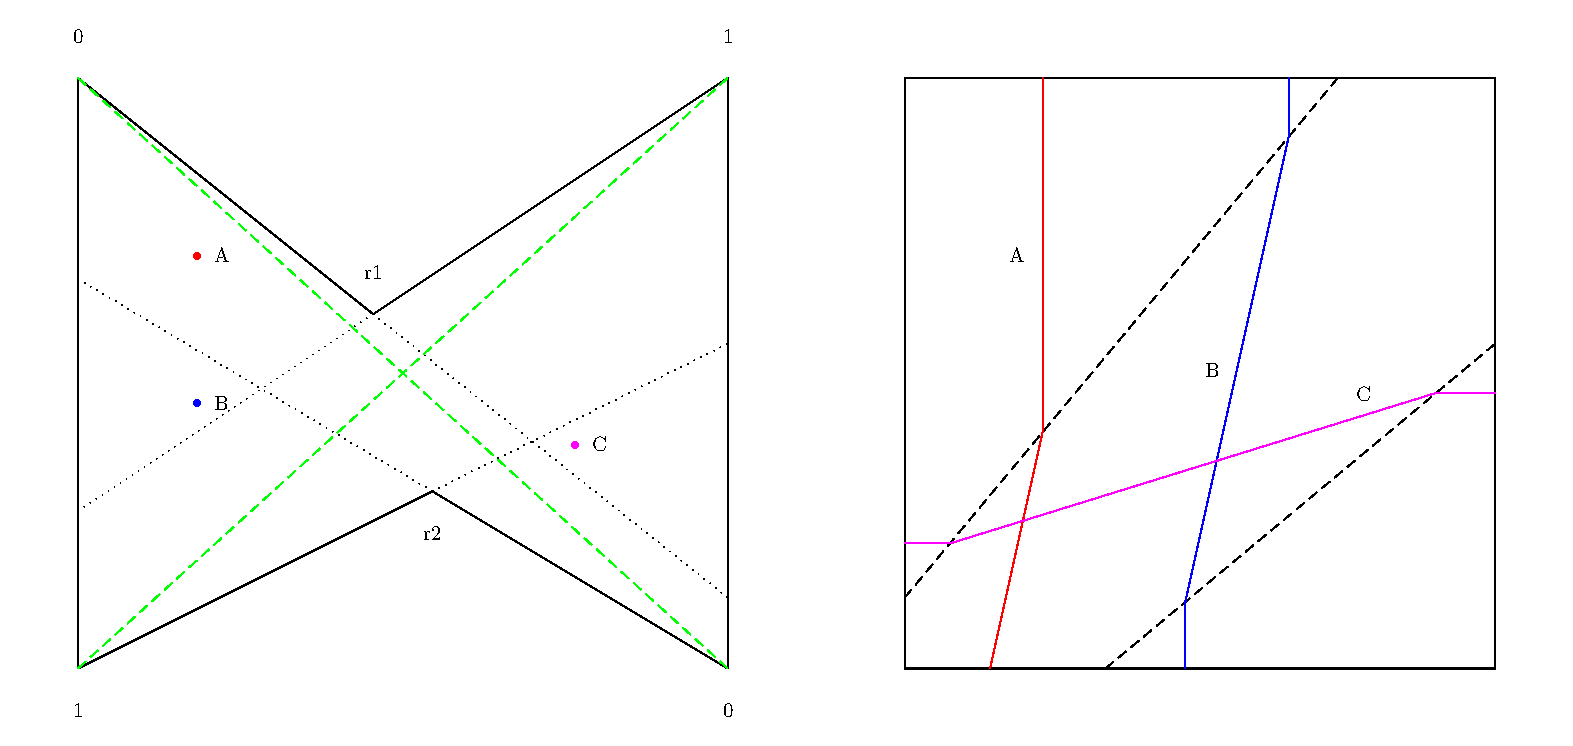
\includegraphics[scale=0.6]{dual}\end{center}
\caption{A 6-gon containing three points (left) and the dual of these
three points (right).}
\figlabel{dual}
\end{figure*}

The dual of a point $p$ in our polygon is defined as follows:  There
is an infinite set of interesting geodesics that contain $p$.  Each of
these geodesics $g$ maps to a dual point $(g_x,g_y)$ as described
above.  The locus of all such points is a (weakly) $x$ and
$y$-monotone curve that joins two points on the boundary of the unit
square. (This latter property can be proved by showing that, if there
is no interesting geodesic containing $w$ (respectively, $x$) and $p$
then there is an interesting geodesic containing $y$ (respectively,
$z$) and $p$.) To obtain $\dual{p}$ we extend this curve into a Jordan
arc by attaching two rays whose slope is 1 ($45^\circ$).

\Figref{dual} shows an example 6-gon containing three points
(left) and the dual of these three points (right).  The dashed lines
in the left figure show the duals of the polygon's two reflex
vertices.  This dualization has the following properties:
\begin{enumerate}
\item For a point $p$, $\dual{p}$ consists of at most five line
segments and can be computed in constant time.

\item For a point $p$, $\dual{p}$ is an $x$ and $y$-monotone Jordan
arc. 

\item If a geodesic $g$ is above (respectvely, below) a point $p$ then
the point $\dual{g}$ is above (respectively, below) the Jordan arc
$\dual{p}$.

\item For two points $p$ and $q$ such that the line through $p$ and
$q$ is not collinear with either reflex vertex, $\dual{p}$ and
$\dual{q}$ have at most one point in common.  I.e., a set of
points dualizes to a set of pseudolines.

\end{enumerate}

Property~3 above implies that our problem of finding an interesting
geodesic with $r'$ red points below it and $b'$ blue points below it
is equivalent to finding an intersection of the $r'$ level in
$\dual{R}$ with the $b'$ level in $\dual{B}$.  Properties~1, 2 and 4
imply that this intersection can be found in $O(n)$ time using the
algorithm of Lo and Steiger.  This completes the proof of:

\begin{thm}
Given a polygon $P$ with $m$ vertices, $k$ of which are reflex, and
containing a set $R$ of $r$ red points and a set $B$ of $b$ blue
points, with $r+b+m=n$, there exists a randomized algorithm that finds
a geodesic $pq$ that simultaneously bisects $R$ and $B$ and runs in
$O(n\log k)$ expected time.
\end{thm}

\section{An \boldmath $\Omega(n\log k)$ Lower Bound}
\seclabel{lower-bound}

In this section we show that the algorithm of the previous section is
optimal when parameterizing the running time only in terms of $n$ and
$k$.  To prove this result, we start with a 1-dimensional problem that
has an $\Omega(n\log k)$ lower bound.

Let $G$ and $Y$ be two sets of distinct integers.  We call an element
$x\in Y$ \emph{odd} (respectively, \emph{even}) if the number of
elements of $G$ less than or equal to $x$ is odd (respectively, even).
Let $Y_o$ denote the set of odd elements in $Y$ and let $Y_e$ denote
the set of even elements in $Y$.  From the work of Yao, it follows
that testing if $|Y_o|=|Y_e|$ requires $\Omega(|Y|\log |G|)$ time in
the algebraic computation tree model.  This is true even if the
elements of $G$ (but not $Y$) are given in sorted order.  We refer to
the problem of testing if $|Y_o|=|Y_e|$ as the \parity\  problem. 


Given an instance of \parity\ we construct a ham-sandwich instance as
follows (see \figref{lowerbound}):  Our blue point set $B$
will have $|Y|+2$ points.  Of these points, $|Y|$ are on the $x$ axis
and take their $x$-coordinate from the elements of $Y$.  Our polygon
$P$ has a series of $|G|+2$ spikes through the $x$-axis such that the
line segment joining the tip of the $i$th spike to the tip of the
$(i+1)$st spike intersects the $x$ axis at the $i$th value of $G$.
These spikes are skinny enough and placed so that they do not
intersect any elements of $G\cup B$.  Such a set of spikes is easy to
compute in $O(|G|)$ time because the elements of $G\cup B$ are
integers and the elements of $G$ are sorted.  We then complete our
polygon into a series of $|G|+2$ chambers as shown in
\figref{lowerbound}.

\begin{figure}[htbp]
\begin{center}\includegraphics[width=3in]{lowerbound}\end{center}
\caption{The lower bound input to a ham-sandwich algorithm.}
\figlabel{lowerbound}
\end{figure}

Our two remaining blue points are placed in the $(|G|+2)$nd chamber in
such a way that any geodesic that separates them and enters another
chamber must pass through the tip of the last spike.  Finally, we
place two red points in the first chamber so that any geodesic that
separates them and enters another chamber must pass through the tip of
the first spike.

Observe that, if we take a geodesic $g$ that separates the two red
points in the first chamber and separates the two blue points in the
last chamber, then the number of blue points above and below $G$ is
$|Y_e|+1$ and $|Y_o|+1$, respectively.  Furthermore, of all the
geodesics that separate the two red points, only those that separate
the two blue points in the final chamber have this property.
Therefore, a ham-sandwich geodesic separates the two blue points in
the final chamber if and only $|Y_e|=|Y_o|$.  Thus, computing a
ham-sandwich geodesic and testing if it separates the two blue points
in the final chamber is sufficient to solve the \parity\ problem.
Since this reduction can be accomplished in $O(|Y|+|G|)$ time and
produces a polygon with $O(|G|)$ reflex vertices we obtain the
following theorem:

\begin{thm}
Given sets $R$ of red points and $B$ of blue points in a simple
polygon $P$ with $k$ reflex vertices, finding a ham-sandwich geodesic
requires $\Omega(n\log k)$ time in the algebraic computation tree
model.
\end{thm}

%%%%%%%%%%%%%%%%%%%%%%%%%%%%%%%%%%%%%%%%%%%%%%%%%%%%%%%%%%%%%%%%%%%%%%%%%%%%%%

\section*{Acknowledgements}

This research was initiated at the McGill Workshop on 
Instance-Based Learning at Bellairs Marine Biology Institute, Jan.
31--Feb.6, 2003.  The authors would like to thank the workshop
organizer Godfried Toussaint and the other workshop
participants, namely, 
   Greg Aloupis,
   David Bremner,
   Vida Dujmovi\'c,
   Jeff Erickson,
   Danny Krizanc,
   Henk Meijer,
   Mark Overmars,
   Tom Shermer,
   Sue Whitesides, 
and
   David Wood for helpful
discussions and for providing a stimulating working environment.  Jeff
Erickson was particularly hepful with the lower bound argument in
\secref{lower-bound}.

\bibliographystyle{abbrv}
\bibliography{ham}

\end{document}

